\documentclass[tikz,border=8pt]{standalone}

\usepackage{tikz}
\usetikzlibrary{arrows.meta, positioning, fit, calc, backgrounds}

\tikzset{
  place/.style={circle, draw, thick, minimum size=12mm, align=center, font=\small},
  transition/.style={rectangle, draw, thick, minimum width=16mm, minimum height=7mm, align=center, font=\small, fill=black!4},
  note/.style={font=\small, align=left},
  phase/.style={rounded corners, draw, dashed, inner sep=6mm, fill=black!2},
  flow/.style={-Latex, thick},
  barrier/.style={very thick, draw=black!55},
}

\begin{document}
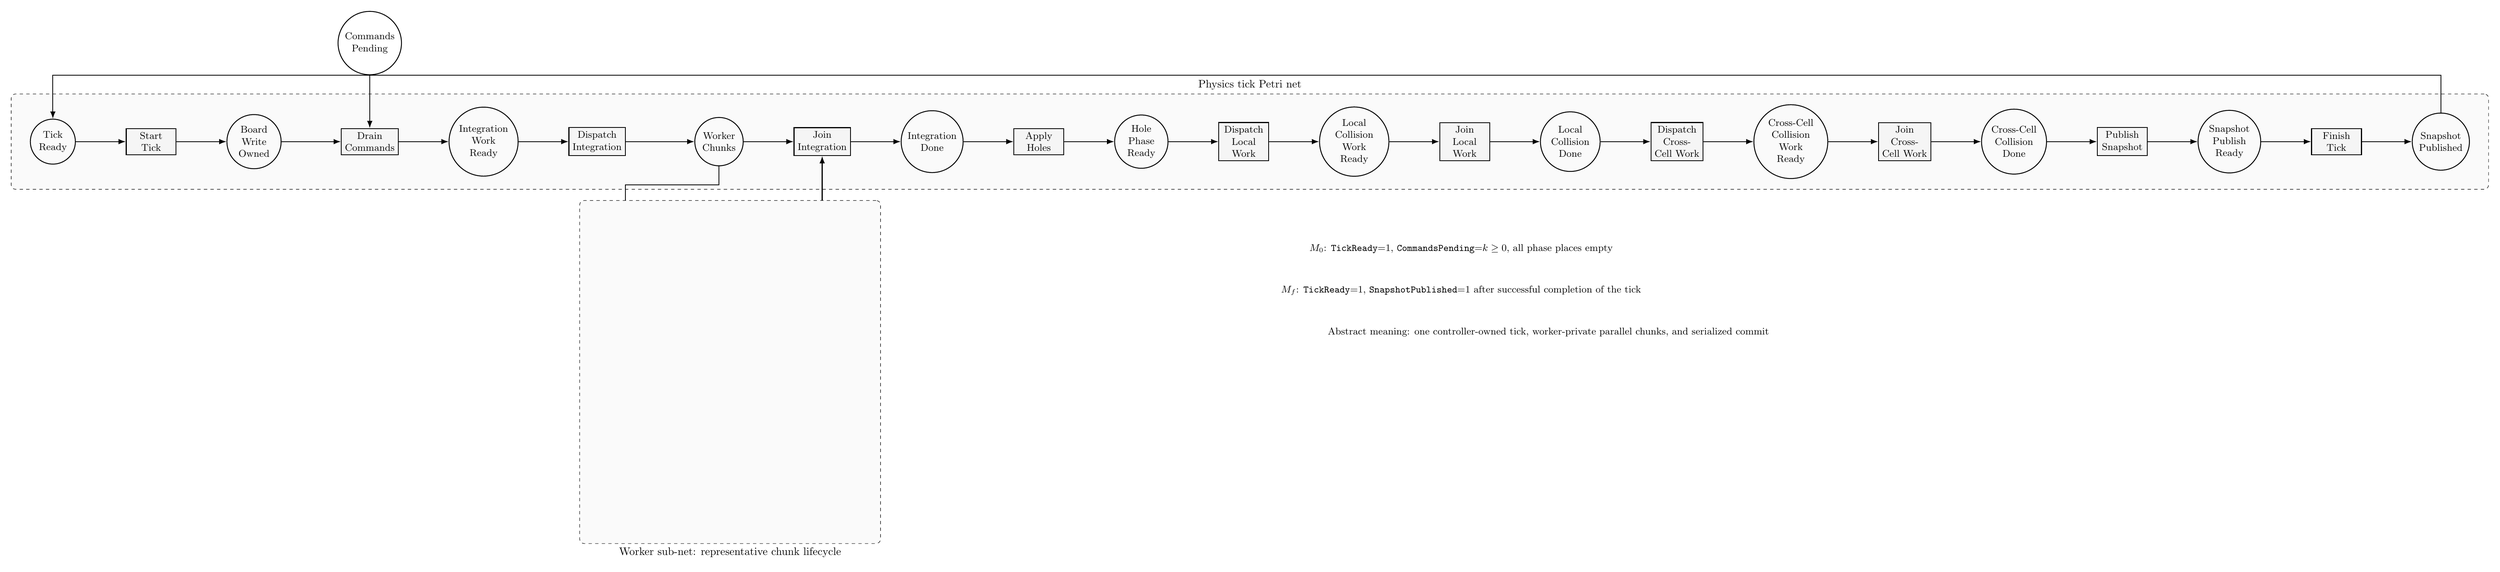
\begin{tikzpicture}[node distance=16mm and 16mm]
  % Main control flow
  \node[place] (tickready) {Tick\\Ready};
  \node[transition, right=of tickready] (starttick) {Start\\Tick};
  \node[place, right=of starttick] (boardowned) {Board\\Write\\Owned};
  \node[transition, right=of boardowned, xshift=3mm] (drain) {Drain\\Commands};
  \node[place, right=of drain] (integrationready) {Integration\\Work\\Ready};
  \node[transition, right=of integrationready] (dispatchi) {Dispatch\\Integration};

  \node[place, right=of dispatchi, xshift=6mm] (iwork) {Worker\\Chunks};
  \node[transition, right=of iwork] (joini) {Join\\Integration};
  \node[place, right=of joini] (integrationdone) {Integration\\Done};
  \node[transition, right=of integrationdone] (holes) {Apply\\Holes};
  \node[place, right=of holes] (holephase) {Hole\\Phase\\Ready};

  \node[transition, right=of holephase] (dispatchc1) {Dispatch\\Local\\Work};
  \node[place, right=of dispatchc1] (localready) {Local\\Collision\\Work\\Ready};
  \node[transition, right=of localready] (joinc1) {Join\\Local\\Work};
  \node[place, right=of joinc1] (localdone) {Local\\Collision\\Done};
  \node[transition, right=of localdone] (dispatchc2) {Dispatch\\Cross-\\Cell Work};
  \node[place, right=of dispatchc2] (crossready) {Cross-Cell\\Collision\\Work\\Ready};
  \node[transition, right=of crossready] (joinc2) {Join\\Cross-\\Cell Work};
  \node[place, right=of joinc2] (crossdone) {Cross-Cell\\Collision\\Done};
  \node[transition, right=of crossdone] (publish) {Publish\\Snapshot};
  \node[place, right=of publish] (snapready) {Snapshot\\Publish\\Ready};
  \node[transition, right=of snapready] (finish) {Finish\\Tick};
  \node[place, right=of finish] (snappub) {Snapshot\\Published};

  % Arcs for the main flow
  \draw[flow] (tickready) -- (starttick);
  \draw[flow] (starttick) -- (boardowned);
  \draw[flow] (boardowned) -- (drain);
  \draw[flow] (drain) -- (integrationready);
  \draw[flow] (integrationready) -- (dispatchi);
  \draw[flow] (dispatchi) -- (iwork);
  \draw[flow] (iwork) -- (joini);
  \draw[flow] (joini) -- (integrationdone);
  \draw[flow] (integrationdone) -- (holes);
  \draw[flow] (holes) -- (holephase);
  \draw[flow] (holephase) -- (dispatchc1);
  \draw[flow] (dispatchc1) -- (localready);
  \draw[flow] (localready) -- (joinc1);
  \draw[flow] (joinc1) -- (localdone);
  \draw[flow] (localdone) -- (dispatchc2);
  \draw[flow] (dispatchc2) -- (crossready);
  \draw[flow] (crossready) -- (joinc2);
  \draw[flow] (joinc2) -- (crossdone);
  \draw[flow] (crossdone) -- (publish);
  \draw[flow] (publish) -- (snapready);
  \draw[flow] (snapready) -- (finish);
  \draw[flow] (finish) -- (snappub);
  \draw[flow] (snappub.north) -- ++(0,12mm) -| (tickready.north);

  % Command queue token feeding the drain transition.
  \node[place, above=of drain, yshift=1mm] (cmds) {Commands\\Pending};
  \draw[flow] (cmds) -- (drain);

  % Worker barrier detail as a readable abstract cluster.
  \node[transition, below=17mm of iwork, xshift=-30mm] (assign) {Assign\\Chunks};
  \node[place, below=of assign] (running) {Worker\\Running};
  \node[transition, below=of running] (complete) {Complete\\Chunk};
  \node[place, below=of complete] (done) {Worker\\Done};
  \node[transition, right=18mm of running] (barrier) {Barrier\\Wait};
  \node[place, right=of barrier] (barriersat) {Barrier\\Satisfied};

  \draw[flow] (iwork.south) -- ++(0,-6mm) -| (assign.north);
  \draw[flow] (assign) -- (running);
  \draw[flow] (running) -- (complete);
  \draw[flow] (complete) -- (done);
  \draw[flow] (done) -- ++(14mm,0) |- (barrier.west);
  \draw[flow] (barrier) -- (barriersat);
  \draw[flow] (barriersat.north) -- ++(0,7mm) -| (joini.south);

  \node[phase, fit=(assign)(running)(complete)(done)(barrier)(barriersat), label=below:{Worker sub-net: representative chunk lifecycle}] {};

  % Annotations
  \node[note, below=22mm of localdone, xshift=-35mm] (initial) {$M_0$: \texttt{TickReady}=1, \texttt{CommandsPending}=$k \ge 0$, all phase places empty};
  \node[note, below=8mm of initial, xshift=0mm] (final) {$M_f$: \texttt{TickReady}=1, \texttt{SnapshotPublished}=1 after successful completion of the tick};
  \node[note, below=8mm of final, xshift=28mm] (semantics) {Abstract meaning: one controller-owned tick, worker-private parallel chunks, and serialized commit};

  % Light grouping around the main pipeline.
  \begin{scope}[on background layer]
    \node[phase, fit=(tickready)(snappub), label=above:{Physics tick Petri net}] {};
  \end{scope}
\end{tikzpicture}
\end{document}
